% https://www.overleaf.com/read/jydxqkkkskzp
% https://github.com/MCG-NKU/NSFC-LaTex
% by Ming-Ming Cheng https://mmcheng.net

\documentclass[12pt]{article}
\usepackage[UTF8]{ctex}
\usepackage{nsfc}
\usepackage{subfigure}
\newcommand{\cmm}[1]{\textcolor[rgb]{0,0.6,0}{CMM: #1}}
\newcommand{\todo}[1]{{\textcolor{red}{\bf [#1]}}}
\newcommand{\myPara}[1]{\paragraph{#1:}}

\graphicspath{{figures/}}


\begin{document}



%%%%%%%%% TITLE

\title{报告正文}

\maketitle

\ContentDes{(一)立项依据与研究内容:}


\NsfcSection{1}{项目的立项依据}{
(研究意义、国内外研究现状及发展动态分析,需结合科学研究发展趋势来论述科学意义;
或结合国民经济和社会发展中迫切需要解决的关键科技问题来论述其应用前景。
附主要参考文献目录);}




\subsection{研究意义}


胃癌是最常见的消化系统肿瘤之一,在癌症中发病率排名第五,致死率排名第四。在我国,胃癌发病率和死亡率均位列第三\cite{1}。2019年我国胃癌新发病例61万例,死亡病例42万例,分别占全球新发和死亡病例的43.9\%和48.6\%\cite{2},严重威胁人民群众的生命健康。胃癌的发生和发展涉及多种因素,包括遗传、环境、生活方式等。尽管近年来的研究取得了一些进展,但我们对胃癌的发病机制仍有很多未知之处。此外,由于早期症状不明显,大部分患者在确诊时已是晚期,这使得治疗更加困难。因此,胃癌防治是我国恶性肿瘤防控面临的重大挑战。我国早期胃癌仅占总确诊的20\%,且胃癌恶性程度较高,我国胃癌患者总体5年生存率不足50\% \cite{3}。目前,胃癌的一线治疗手段以化疗为主,人表皮生长因子受体-2(human epidermal growth factor receptor 2, HER2)阳性患者可联用曲妥珠单抗\cite{4}。虽然曲妥珠单抗、雷莫芦单抗等靶向药物已投入临床应用,但相关靶点阴性的患者药物选择有限,疗效欠佳。因此寻找其他胃癌特异性靶点,开发更具特异性的疗法对提高临床响应率、改善进展期胃癌患者预后十分关键。

嵌合抗原受体T细胞(Chimeric Antigen Receptor T-cell, CAR-T)免疫疗法目前是治疗肿瘤的新疗法,主要应用于血液肿瘤\cite{5}。CAR-T细胞免疫疗法通过工程化改造T细胞抗原识别区域,能够直接识别肿瘤细胞表面抗原,特异性杀伤肿瘤细胞,减少治疗对机体正常细胞的损伤。受限于实体瘤内的抑制性肿瘤微环境,CAR-T疗法目前在实体瘤领域进展较慢。近年来,细胞免疫疗法已由单纯CAR-T疗法逐渐发展为联合治疗,如联合放化疗、免疫检查点抑制剂等,为治疗实体瘤提供了新的方向。因此,以CAR-T为代表的细胞免疫疗法在实体瘤领域中具有很好的应用前景。CAR-T技术将抗体的单链可变区域与T细胞表面受体结合,负责识别靶抗原;连接铰链区将抗体嵌合于细胞膜上;在胞内区域构建共刺激因子和CD3信号域,使产生的刺激信号传导到下游通路,从而激活T细胞并发挥其杀伤功能\cite{6}。

紧密连接是上皮细胞和内皮细胞的主要连接方式\cite{7},紧密连接蛋白(Claudin, CLDN)表达在细胞膜上,是细胞间紧密连接的重要组成部分\cite{8}。CLDN家族蛋白在不同组织中表达程度不同,其中CLDN18特异性表达在食管和胃黏膜上\cite{9}。Fassan等研究者通过免疫组化染色发现,在523例胃癌患者中,29.4\%的原位肿瘤和34.1\%的转移灶高表达CLDN \cite{10}。CLDN18.2是CLDN18的一种亚型,在胃癌及其转移灶中稳定表达,而在正常胃组织中不表达\cite{11}。有研究表明,86.7\%的胃癌组织表达CLDN18.2,且73.3\%的组织高表达CLDN18.2 \cite{12}。综上,CLDN18.2特异地表达在胃癌肿瘤细胞膜上,参与肿瘤细胞的增殖和转移,以CLDN18.2为靶点设计CAR-T疗法对胃癌治疗颇具意义。

近年来,已经有许多研究者聚焦于CLDN18.2为靶点的CAR-T疗法。Zonghai Li等首次构建了以CLDN18.2为靶点的CAR-T,并在小鼠皮下瘤模型中验证了靶向CLDN18.2的CAR-T的有效性和持久性12。Lin Shen等开展了一项CLDN18.2 CAR-T细胞治疗消化道肿瘤的一期临床研究。其中,胃腺癌患者的客观缓解率和疾病控制率分别达到57.1\%和75\%\cite{13}。

上皮细胞粘附分子(epithelial cell adhesion molecule, EpCAM)是一种表达在上皮细胞的跨膜糖蛋白,在正常细胞中起到维持细胞间黏附、参与细胞信号传导何调控细胞增殖等功能\cite{14}。然而,EpCAM也在多种肿瘤组织中过度表达,其中包括胃癌\cite{15}。EpCAM在胃癌中的高表达水平与预后不良、肿瘤的恶性程度及患者的生存率下降相关\cite{16}。靶向EpCAM的CAR-T疗法已投入Ⅰ期临床研究以检验其安全性和有效性(NCT05028933)。

在提高CAR-T疗法有效性的同时,研究者也十分关注CAR-T疗法的安全性。CAR-T的毒性主要有细胞因子释放综合征(cytokine release syndrome, CRS)和神经毒性,但在临床转化前,动物实验均未预测到这两种不良反应\cite{17}。这两种毒性都是由T细胞快速活化后大量分泌的细胞因子引起,高肿瘤负荷和CAR-T快速扩增与较高等级的CRS相关\cite{18}。CRS患者通常在CAR-T治疗的第一周内表现为发热、低血压和呼吸功能不全\cite{19,20},神经毒性可表现为谵妄、癫痫或急性脑水肿\cite{21}。严重神经毒性或CRS引起的多器官衰竭可导致患者死亡。此外,有研究发现,CAR-NK中CAR的激活促进CAR靶抗原从肿瘤细胞转移到NK细胞中,诱导NK细胞自我识别和自我杀伤,NK细胞出现耗竭,削弱CAR-NK治疗的疗效\cite{22}。为预防和管理这些不良反应,研究者们正在探索多种策略,包括优化CAR结构、使用免疫调节剂以及开发更安全的治疗方案。Sadelain 等研究者为预防CAR-T毒性,设计了共同识别两种抗原的“与门(AND-gate)”CAR-T,并在小鼠模型中比较AND-gate CAR-T和其他逻辑门控系统,验证了AND-gate CAR-T的有效性和安全性\cite{23}。

本项目在设计靶点的同时更加关注CAR-T治疗的安全性,希望能够减少毒性和CAR细胞自我杀伤。本项目拟采用AND-gate逻辑门控策略,共同识别EpCAM和CLDN18.2这两种胃癌特异性抗原。这种设计有助于实现对胃部肿瘤细胞的精确识别与攻击,仅在两种抗原同时存在时,CAR-T细胞才会被激活并发挥杀伤作用。这显著降低了对仅表达单一抗原的正常细胞的误伤风险,从而提高了疗法的安全性。此外,双靶点设计还有助于应对胃癌的抗原异质性问题。在确保安全性的同时,这种策略使得CAR-T细胞能够更有效地识别和攻击那些同时表达两种抗原的不同表型的胃癌细胞,从而提高治疗的有效性。



\subsection{国内外相关工作}

\textbf{缺少了这部分,需要挪一部分单独写在这里。}

{
\bibliographystyle{unsrt}
\bibliography{Cmm}
}


%%%%%%%%%%%%%%%%%%%%%%%%%%%%%%%%%%%%%%%%%%%%%%%%%
\NsfcSection{2}{项目的研究目标、研究内容,以及拟解决的关键科学问题}{
(此部分为重点阐述内容);}

\subsection{研究目标}

本课题旨在设计CLDN18.2和EpCAM双靶点的CAR-T细胞疗法,为HER2、VEGF等传统靶点阴性患者提供高特异性的安全免疫治疗方案。这种双靶点CAR-T疗法能够更好地应对肿瘤异质性问题,扩大治疗覆盖范围,并提高治疗的有效性和特异性。AND-gate CAR-T技术是一种独特的CAR-T治疗方法,它为胃癌治疗提供了全新的思路,并有望推动CAR-T细胞治疗领域的不断发展。此外,本项目的成果也将为其他实体瘤的治疗提供有价值的参考,拓展细胞免疫治疗的应用领域。总之,以CLDN18.2和EpCAM为双靶点的AND-gate CAR-T治疗胃癌在促进个体化治疗、推动免疫治疗创新、解决免疫治疗面临的挑战等方面都具有深远的意义,为临床实践带来了新的治疗思路。




\subsection{研究内容}

\textbf{本项目的研究内容在之前没有安排人写,分工一下}

\subsection{拟解决的关键科学问题}

\textbf{同,需补充}

本项目基于上述研究和文献综述,提出以下假设:以CLDN18.2和EpCAM为双靶点的AND-gate CAR-T可以通过??通路,诱导??,最终发挥肿瘤杀伤作用,为胃癌免疫治疗提供安全性更高的临床策略。

\NsfcSection{3}{拟采取的研究方案及可行性分析}{
(包括研究方法、技术路线、实验手段、关键技术等说明);}


\subsection{拟采取的技术路线}

\subsubsection{细胞株构建}

在完成所需CAR的序列设计之后,需要为递送到细胞并在其中成功表达构建递送载体。慢病毒是目前构建CAR-T广泛使用的递送工具,能提供6.5k大小的基因插入,因其在T细胞中较于一般质粒载体相对有效的侵染效率而得以推广。但由于慢病毒载体递送DNA过程中插入位点的随机性和潜在的致癌性,以及多病毒侵染的困难性,其应用范围受到限制。DNA转座子是用于基于递送的一类非病毒载体,它由两个功能部分组成,即转座序列和转座酶,二者由分离的或同一质粒表达。表达后,转座酶特异性识别转座DNA两端的末端识别序列,将其切离并携带直至在染色体上寻找并插入到另一个位点。转座子系统用于CAR-T细胞的构建相对于病毒载体而言具有包括高载体容量、低免疫反应在内的多种优势,但其在CAR-T中的应用因其转座位点的不可控性和转座发生的重复性也受到限制。为了解决转座系统的这些缺陷,我们针对设计了Tet-on系统搭载的IRES-PBase表达盒,来实现对效应时间的有效控制,从而降低多次转座可能带来的潜在的肿瘤诱导风险。

\subsubsection{质粒构建}
对于CLDN18.2和EpCam的敲除质粒,使用pAAV-U6SagRNA-CAG-Sacas9-puro作为模板,使用 NEBuilder HiFi DNA Assembly Cloning Kit将T2A-BFP无缝克隆至sacas9后,以实现对敲除成功的细胞的有效标记,同时选取在CLDN18.2的第2/3个外显子位置选取适当的gRNA以确保对目标基因的有效敲除。对于嵌合抗原受体表达质粒,针对被转染细胞设计克隆至不同质粒载体。对于HDFa细胞,使用V8-MCS-puro载体,使用KpnI切开载体并使用NEBuilder HiFi DNA Assembly Cloning Kit将附带红色荧光的CAR以及受5XUAS转录调控的eGFP克隆至载体上。对于转染T细胞的质粒使用piggybac-TetO-puro载体,分别在其中加入两个CAR和转录因子调控序列,然后最后加入IRES-PB转座酶,以确保质粒的完整性。

\begin{figure}[htbp]
	
	\centering
	\subfigure[第1个质粒]{
		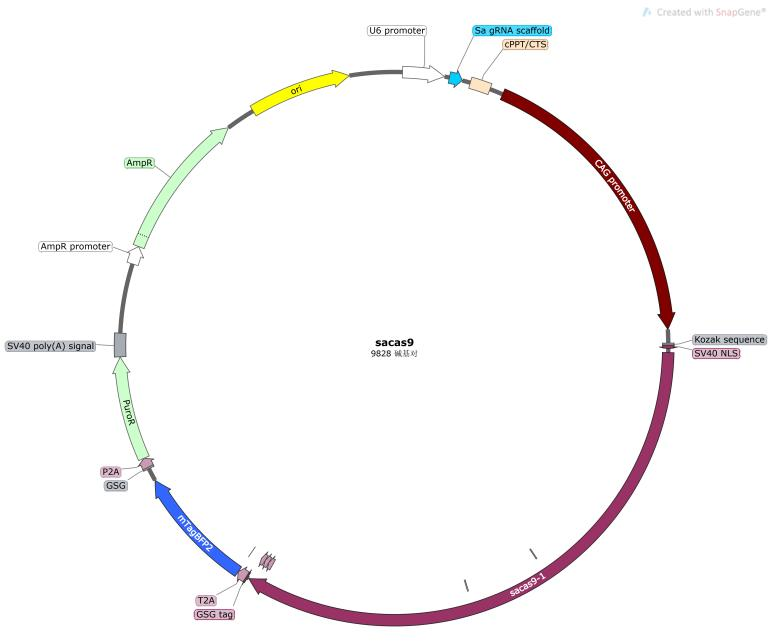
\includegraphics[width=6.5cm]{figures/sacas9}
		%\caption{fig1}
	}
	\quad
	\subfigure[第2个质粒]{
		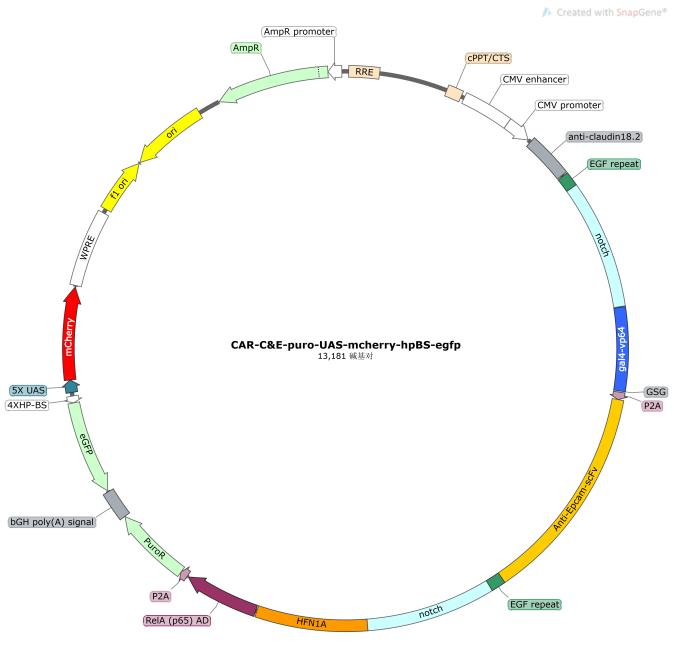
\includegraphics[width=6.5cm]{figures/carce}
	}
	\quad
	\subfigure[第3个质粒]{
		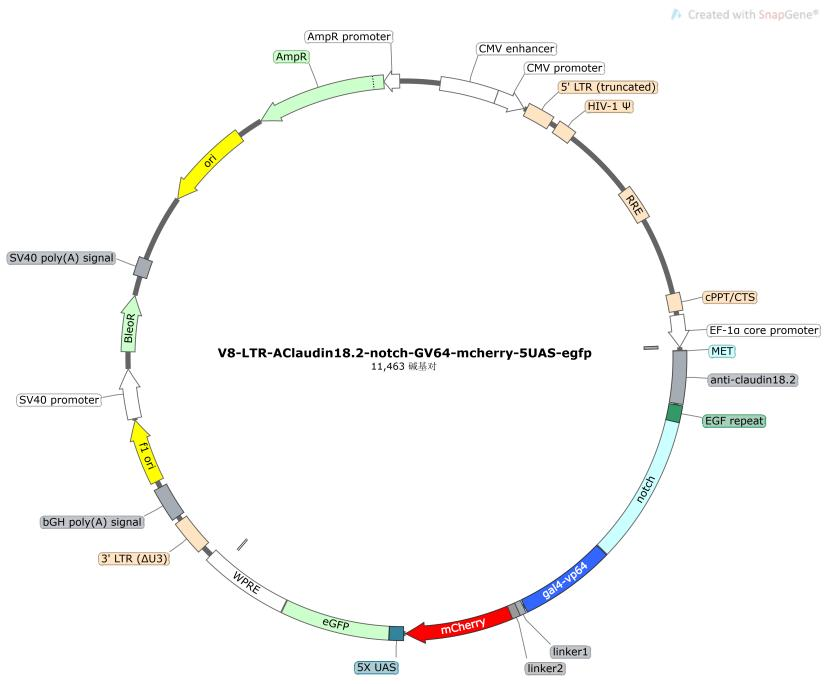
\includegraphics[width=6.5cm]{figures/V8}
	}
	\quad
	\subfigure[第4个质粒]{
		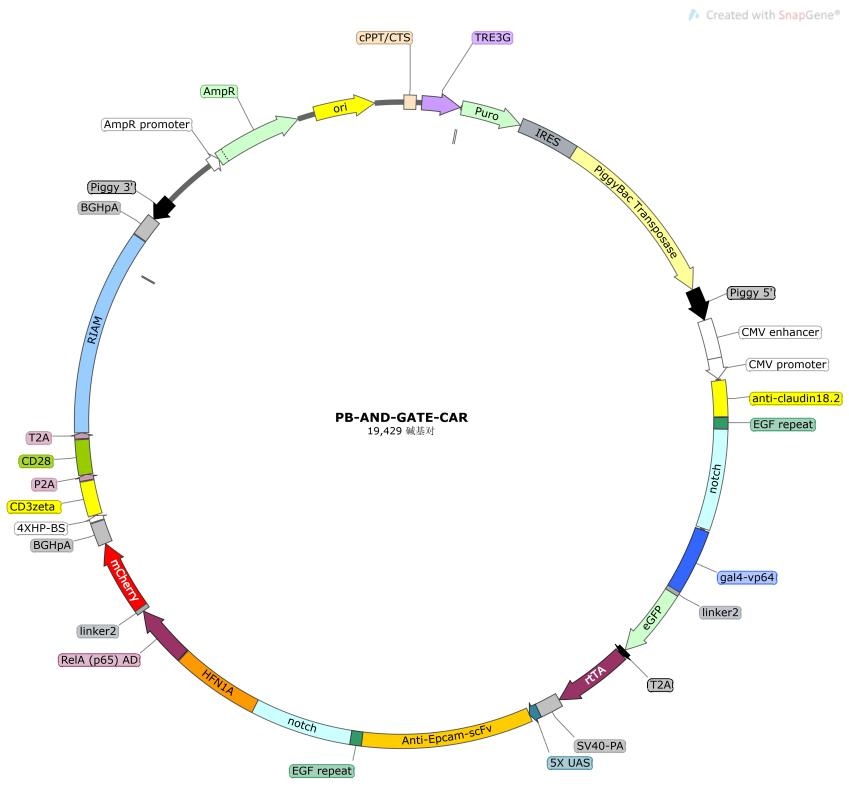
\includegraphics[width=6.5cm]{figures/pb}
	}
	\\[3pt]
	\caption{\quad Group 5的几何模型展示}
	\label{model}
\end{figure}

\subsubsection{CAR-HDFa细胞株构建}

构建靶向CLDN18.2的CAR-HDFa细胞株以验证Anti-CLDN18.2-Syn-notch CAR的功能。

\textbf{细胞培养:}根据制造商提供的说明,从成人皮肤分离的原代人真皮成纤维细胞HDFa,在不存在抗生素和抗真菌药物的情况下,在具有低血清生长补充剂的培养基RPMI 1640中培养。
将细胞维持在37°C、含5\% $\mathrm{CO}_2$的湿润气氛中,并使用0.25\%胰蛋白酶-0.1\%EDTA(v/v)常规传代。

\textbf{质粒转染和筛选:}对于HDFA、SNU-601,用Lipofectamine 3000(Life Technologies)转染质粒(300 ng)用4ug/ml浓度的嘌呤霉素选择细胞,并在转染后5至7天收集细胞。对于Jurkat T和人原代CD4/CD8+ T细胞,我们用Lipofectamine 3000转染质粒(500 ng)后用多西环素(1pM)加入完全培养基,1天之后额外加入2ug/ml浓度的嘌呤霉素选择细胞,并在转染后5至7天收集细胞。

\subsubsection{动物模型和类器官构建}

\begin{figure}[h]
	\centering
	\begin{overpic}[width=0.6\columnwidth]{organ.jpg}
	\end{overpic}
	\caption{缺少图注}
	\label{organ}
\end{figure}

\subsubsection{Notch样受体理论可行性验证}

为了验证Syn-Notch样受体是否能够在接触抗原后,通过抗原-抗体识别裂解受体,使得连接于受体上的转录因子(TF)通过剪切作用脱离受体,进入下游表达回路中,设计一组对照试验,在相互间不存在免疫反应的两类细胞上分别构建胃癌细胞特异性抗原Claudin18和能够特异性识别该抗原的anti-CLDN18 Notch样受体。其中,起“信号接收”作用的Receiver cell选择人源成纤维细胞系HDFa,起“信号发送”作用的Sender cell选择高表达Claudin18的胃癌细胞系SNU-601。

Receiver cell的Notch样受体上连接的转录因子为Gal4-VP64。Gal4-VP64 转录激活结构域工作可靠,是一种常用的人工转录激活因子,由酵母Gal4 DNA结合结构域和4个串联的疱疹病毒VP16转录激活结构域组合而成。Gal4 DNA结合结构域可以特异性识别其靶序列UAS(上游激活序列),从而带来VP16转录激活结构域,实现对下游基因的转录激活。VP16转录激活结构域包含一个强大的促进子激活结构域,可以募集RNA聚合酶及其共激活因子,启动基因转录。由Gal4-VP64组成的转录因子能够特异性地开启下游GFP的表达。

Sender cell构建为过表达蓝色荧光蛋白BFP的SNU-601细胞系。Claudin18在野生型SNU-601中高表达。另制备Claudin18敲除株SNU-601 ΔCLDN18。

当Receiver cell表面的Notch样受体接触到Sender cell表面高表达的Claudin18时,若Notch可按照结构的理论功能正常工作,包括(1)抗原-抗体正确结合(2)Notch样受体能够正常裂解使得转录因子Gal4-VP64被剪切掉落,则可以开启GFP的合成通路,使HDFa细胞发绿色荧光。对于前者的验证,使用空白对照;对于后者的验证,在一组阴性对照中加入一定浓度能抑制受体裂解的γ-分泌酶抑制剂DAPT,阻断Notch裂解。

对照设置为:CAR-gal4-mcherry+ GFP plasmid + sacas9(with/without grna)-bfp

(1)空白组:HDFa-Notch-GFP

(2)实验组:HDFa-Notch-GFP + SNU-601-BFP

(3)阴性对照1:HDFa-Notch-GFP + SNU-601 ΔCLDN18-BFP

(4)阴性对照2:HDFa-Notch-GFP + SNU-601-BFP + 1mM DAPT

(5)阳性对照:HDFa-文献中经过验证的Notch-GFP+ SNU-601-BFP


在FM完全培养基中于37℃和5\% $\mathrm{CO}_2$下共培养HDFa细胞和SNU-601细胞24 hr,控制接种细胞密度为$1\times 10^5 \ \mathrm{cell / cm}^2$。使用流式细胞仪统计不同组内GFP荧光信号的强度,应观察到除实验组外,空白组和阴性对照组的GFP强度很低。在荧光共聚焦显微镜下观察各组细胞,应在实验组和阴性对照组中仅观察到发蓝色荧光的SNU-601细胞,而在实验组中可以同时观察到发蓝色荧光和绿色荧光的细胞。

\begin{figure}[h]
	\centering
	\begin{overpic}[width=0.8\columnwidth]{41.jpg}
	\end{overpic}
	\caption{缺少图注}
	\label{organ}
\end{figure}

\begin{figure}[h]
	\centering
	\begin{overpic}[width=0.6\columnwidth]{42.jpg}
	\end{overpic}
	\caption{缺少图注}
	\label{organ}
\end{figure}

\subsubsection{双Syn-Notch受体的正交性验证}

\textbf{构建双synNotch受体细胞株:}分别构建双synNotch受体表达质粒,使anti-CLDN18 synNotch连接Gal4-VP64转录激活域,控制mCherry报告基因表达;anti-EpCAM synNotch连接HNF1α转录激活域,控制GFP报告基因表达。转染质粒至人源成纤维细胞(HDFa),获得双synNotch受体细胞株,如图\label{5}A所示。

\textbf{验证双synNotch受体功能正交:}分别用不同SNU-601细胞(SNU-601-$\Delta$CLDN18、SNU-601-$\Delta$EpCAM、SNU-601-WT)与双synNotch受体HDFa以1:1的比例共培养。在96孔组织培养板中细胞后,将细胞400×g离心1 min以迫使细胞相互作用,24小时后分析培养物的活化标志物,如图\label{5}A所示。

\begin{figure}[h]
	\centering
	\begin{overpic}[width=0.8\columnwidth]{5.jpg}
	\end{overpic}
	\caption{(A)同时表达具有Gal4-VP64胞内结构域和mCherry报告基因的抗CLDN18 synNotch受体和具有HNF1α胞内结构域和GFP报告基因的抗EpCAM synNotch受体的人源成纤维细胞。(B)受不同SNU-601细胞刺激后双synNotch受体细胞的报告基因激活情况。若双synNotch受体功能正交,则仅在对应的抗原刺激下可观察到单一报告基因的激活,而在双抗原刺激下可以同时观察到两个报告基因的激活。}
	\label{5}
\end{figure}

\subsubsection{双synNotch受体级联AND-gate构建}

\textbf{构建双synNotch受体T细胞株:}
分别对Jurkat T、CD4+、CD8+细胞进行工程化,使其细胞膜上表达anti-CLDN18 synNotch受体,且当anti-CLDN18 synNotch受体受到配体刺激时,能使Gal4-VP64-GFP转移至核内,并诱导带mcherry荧光标记的anti-EpCAM synNotch受体在细胞膜上的表达。当anti-EpCAM synNotch受体收到配体刺激时,转录因子HNF1α转移到核内,诱导CD3,CD28表达,从而进一步诱导T细胞活化,如图\label{6}A所示。

\textbf{确认双synNotch受体级联AND-gate的形成:}
将SNU-601-WT细胞与双synNotch受体T细胞按照1:10的比例在37°C和5\% CO2下共培养72小时,用荧光共聚焦显微观察不同刺激时间下2种荧光蛋白(GFP和mCherry)的空间分布,绘制2种荧光强度随时间的变化曲线,如图\label{6}B所示。

\textbf{T细胞活化鉴定:}
将SNU-601-WT细胞与双synNotch受体T细胞按照1:10的比例在37°C和5\% $\mathrm{CO}_2$下共培养,不同刺激时间(24 hr,48 hr,72 hr,96 hr)后流式检测并比较mCherry(+)和mCherry(-)T细胞胞内CD3,CD28表达情况,并用qPCR测定T细胞活化标志物表达量。

\begin{figure}[h]
	\centering
	\begin{overpic}[width=0.8\columnwidth]{6.jpg}
	\end{overpic}
	\caption{双synNotch受体级联AND-gate示意图。(A)T细胞表达anti-CLDN18 Syn-Notch连接Gal4-VP64-GFP转录激活域,即Gal4-VP64上连接着绿色荧光报告基因,当识别CLDN18时,绿色荧光随Gal4-VP64转移到核内,并控制anti- EpCAM synNotch-HNF1α-mCherry的表达。anti-EpCAM synNotch-HNF1α-mCherry被表达并运输至T细胞膜表面,细胞膜处出现红色荧光。(B)预期的荧光强度随时间变化曲线。}
	\label{6}
	
\end{figure}

\subsubsection{AND-gate CAR-T的体外安全性、有效性}

构建含有级联AND-gate的人原代CD4+ T细胞和CD8+ T细胞为CAR-T细胞。(第一个car gfp 第二个car mecherry 最后效应带bfp)靶细胞只有同时存在EpCAM和CLDN18两种抗原,才会激活代CarT细胞。

\textbf{体外有效性验证:}

选取胃印戒细胞癌snu601细胞株为靶细胞。将原代CD4+ CAR-T细胞和CD8+ CAR-T细胞与SNU-601-ΔCLDN18、SNU-601-ΔEpCAM或野生型SNU-601(WT- SNU-601)细胞按照1:10的比例共培养,条件为1640完全培养基(含10\%血清,1\%双抗), 37°C和5\% CO2,时间为72 hr,snu601细胞的初始接种密度为$1\times 10^5 \ \mathrm{cell / cm}^2$。

对于CD4+ CAR-T细胞:

(1)流式细胞术检测不同共培养体系下的BFP荧光阳性的比例。

(2)取细胞上清液进行elisa检测细胞因子,如IL-13、IL-12、IL-6、IL-2、IL-4、IL-8等及RANTES、GMCSF、MIP-1a、IFNγ、TNFα等。 

对于CD8+ CAR-T细胞:

(1)流式细胞术检测不同共培养体系下的BFP荧光阳性的比例。

(2)正向和侧向散射流式细胞图,圈门观察SNU-601细胞群的数量减少情况。示意图如下说明:T细胞体积较小可以视为左下角群,右上角群为效应细胞群,这群细胞的比例即位肿瘤细胞的存活比例。

\begin{figure}[h]
	\centering
	\begin{overpic}[width=0.6\columnwidth]{7.jpg}
	\end{overpic}
	\caption{缺少图注}
	\label{6}
	
\end{figure}


\textbf{体外安全性验证:}选取人源胃上皮细胞系细胞为靶细胞。将原代CD4+ CAR-T细胞和CD8+ CAR-T细胞与选取人源HDFa细胞共培养,ELISA检测CD4+ CAR-T细胞上清的细胞因子,流式细胞术检测CD8+ CAR-T细胞共培养后HDFa细胞的存活比例。

\subsubsection{AND-gate CAR-T的体内安全性、有效性}

进一步评估具备级联AND-gate的CAR T在肿瘤治疗方面的安全性和有效性,检测CD4+ CAR T 细胞和CD8+ CAR T细胞在双抗原异种移植模型中控制肿瘤生长的能力。

\textbf{体内有效性验证:}

小鼠使用遗传背景为NOD并携带有联合免疫缺陷突变(scid)和IL2R的γ链完全敲除突变(IL2rgnull)的重度免疫缺陷小鼠NSG小鼠。

实验分组a:在NSG小鼠的左侧腋下(flank的翻译)皮下植入SNU-601细胞系,在NSG小鼠的右侧腋下皮下植入SNU-601-ΔEpCAM细胞系。

实验分组b:在NSG小鼠的左侧腋下皮下植入SNU-601细胞系,在NSG小鼠的右侧腋下皮下植入将SNU-601-ΔCLDN18细胞系。

皮下植入四天后,将CD4+ CAR-T细胞和CD8+ CAR-T细胞或未经转导的CD4+和CD8+ T细胞静脉注射到NSG小鼠体内,注射后12h观察GFP和BFP荧光比例,并在16天内测量肿瘤大小,计算肿瘤体积,绘制肿瘤体积变化曲线和生存曲线。理论上SNU-601细胞系植入组小鼠具有明显优于ΔEpCAM或ΔCLDN18的生存曲线。CarT清除缺乏EpCAM或BFP抗原的肿瘤能力减弱,肿瘤生长不受控制。


\textbf{体内安全性验证:}

对于非荷瘤小鼠模型,使用转染荧光素酶的 CD4+ CAR-T(CAR-T-FLuc)细胞和CD8+ CAR-T细胞尾静脉注射到NSG、B6 及 BALB/c三种背景的小鼠体内,于给药后不同时间点采用活体成像的方法检测 CAR-T-FLuc 细胞分布情况,并在给药后 3 h 和 2、7、14、28d 解剖动物,取血液、心脏、肝脏、脾脏、肺脏、肾脏、脑、睾丸、附睾、子宫、卵巢、胃、十二指肠、骨髓、脂肪、骨骼肌,QPCR 方法检测 CAR-T-FLuc 细胞在外周血及上述组织器官中的分布情况。注射后30天内监测小鼠的体重,外周血中红细胞数。观察CAR-T细胞是否会导致小鼠出现严重的体重减轻,贫血等并发症。以及各器官中CAR-T细胞的浸润比例。


对于荷瘤小鼠模型,在NSG小鼠的腋下皮下植入SNU-601细胞系,建立肿瘤模型,之后给予 CAR-T-FLuc 细胞,并采用与非荷瘤小鼠相同的检测方法考察 CAR-T-FLuc 细胞在活体和各组织脏器不同时间点的表达。观察CAR-T细胞是否会导致小鼠出现严重的体重减轻,贫血等并发症。


\subsection{可行性分析}


\NsfcSection{4}{本项目的特色与创新之处;}{}

\textbf{这部分还没安排}

\NsfcSection{5}{年度研究计划及预期研究结果}{
(包括拟组织的重要学术交流活动、国际合作与交流计划等)。}

\textbf{问一下老师要不要写这部分}

\subsection{年度研究计划}


\subsection{预期研究成果}


%%%%%%%%%%%%%%%%%%%%%%%%%%%%%%%%%%%%%%%%%%%%%%%%%
\ContentDes{(二)研究基础与工作条件}

\textbf{安排谁写一下}

\NsfcSection{1}{研究基础}{
(与本项目相关的研究工作积累和已取得的研究工作成绩);}

\subsection{工作基础1}

\subsection{工作基础2}



\NsfcSection{2}{工作条件}{
(包括已具备的实验条件,尚缺少的实验条件和拟解决的途径,
包括利用国家实验室、
国家重点实验室和部门重点实验室等研究基地的计划与落实情况);}

\textbf{问一下老师要不要写这部分}

\myPara{经费和硬件条件方面}我们


\myPara{人员方面}我们

\myPara{国内外合作方面} 我们


\NsfcSection{3}{正在承担的与本项目相关的科研项目情况}{
(申请人和项目组主要参与者正在承担的与本项目相关的科研项目情况,
包括国家自然科学基金的项目和国家其他科技计划项目,
要注明项目的名称和编号、经费来源、起止年月、与本项目的关系及负责的内容等);}


%%%%%%%%%%%%%%%%%%%%%%%%%%%%%%%%%%%%%%%%%%%%%%%%%
\ContentDes{(三) 其他需要说明的问题}



\NsfcSection{1}{}{
申请人同年申请不同类型的国家自然科学基金项目情况
(列明同年申请的其他项目的项目类型、项目名称信息,
并说明与本项目之间的区别与联系)。}


\NsfcSection{2}{}{
具有高级专业技术职务(职称)的申请人或者主要参与者是否存在
同年申请或者参与申请国家自然科学基金项目的单位不一致的情况;
如存在上述情况,列明所涉及人员的姓名,
申请或参与申请的其他项目的项目类型、项目名称、单位名称、
上述人员在该项目中是申请人还是参与者,并说明单位不一致原因。}



\NsfcSection{3}{}{
具有高级专业技术职务(职称)的申请人或者主要参与者是否具有
高级专业技术职务(职称)的申请人或者主要参与者是否存在与正
在承担的国家自然科学基金项目的单位不一致的情况;如存在上述情况,
列明所涉及人员的姓名,正在承担项目的批准号、项目类型、项目名称、
单位名称、起止年月,并说明单位不一致原因。}


\NsfcSection{4}{}{其他。}

无


\end{document}
